% Deze template is gemaakt door Fons van der Plas (f.vanderplas@student.ru.nl) voor het publiek domein en mag gebruikt worden **zonder vermelding van zijn naam**.
% This template was created by Fons van der Plas (f.vanderplas@student.ru.nl) for the public domain, and may be used **without attribution**.
\documentclass{article}
\usepackage[utf8]{inputenc}     % for éô
\usepackage[english]{babel}     % for proper word breaking at line ends
\usepackage[a4paper, left=1.5in, right=1.5in, top=1.5in, bottom=1.5in]{geometry}
                                % for page size and margin settings
\usepackage{graphicx}           % for ?
\usepackage{amsmath,amssymb}    % for better equations
\usepackage{amsthm}             % for better theorem styles
\usepackage{mathtools}          % for greek math symbol formatting
\usepackage{enumitem}           % for control of 'enumerate' numbering
\usepackage{listings}           % for control of 'itemize' spacing
\usepackage{todonotes}          % for clear TODO notes
\usepackage{hyperref}           % page numbers and '\ref's become clickable
\usepackage{etoolbox}
\usepackage{lipsum}   % for filler text
\usepackage{setspace}
\usepackage{caption}
\usepackage{subcaption}
\usepackage{xcolor}

\AtBeginEnvironment{quote}{\singlespacing\small}

\definecolor{codegreen}{rgb}{0,0.6,0}
\definecolor{codegray}{rgb}{0.5,0.5,0.5}
\definecolor{codepurple}{rgb}{0.58,0,0.82}
\definecolor{backcolour}{gray}{0.95}
 
\lstdefinestyle{mystyle}{
    backgroundcolor=\color{backcolour},   
    commentstyle=\color{codegreen},
    keywordstyle=\color{magenta},
    numberstyle=\tiny\color{codegray},
    stringstyle=\color{codepurple},
    basicstyle=\ttfamily\footnotesize,
    breakatwhitespace=false,         
    breaklines=true,                 
    captionpos=b,                    
    keepspaces=true,                 
    numbers=left,                    
    numbersep=5pt,                  
    showspaces=false,                
    showstringspaces=false,
    showtabs=false,                  
    tabsize=2
}

\lstset{style=mystyle}

%%%%%%%%%%%%%%%%%%%%%%%%%%%%%%%%
%% SET TITLE PAGE VALUES HERE %%
%%%%%%%%%%%%%%%%%%%%%%%%%%%%%%%%
%             ||               %
%             ||               %
%             \/               %

\def\thesistitle{Convolutional Neural Networks applied to Keyword Spotting using Transfer Learning}
\def\thesissubtitle{Why Transfer learning is worth a try}
\def\thesisauthorfirst{Christoph}
\def\thesisauthorsecond{Schmidl}
\def\thesisauthorstudentnumber{s4226887}
\def\thesisauthoremail{c.schmidl@student.ru.nl}
\def\thesissupervisorfirst{dr. L.F.M. }
\def\thesissupervisorsecond{ten Bosch}
\def\thesissecondreaderfirst{prof. dr. Louie}
\def\thesissecondreadersecond{Duck}
\def\thesisdate{\today}


%             /\               %
%             ||               %
%             ||               %
%%%%%%%%%%%%%%%%%%%%%%%%%%%%%%%%
%% SET TITLE PAGE VALUES HERE %%
%%%%%%%%%%%%%%%%%%%%%%%%%%%%%%%%


%% FOR PDF METADATA
\title{\thesistitle}
\author{\thesisauthorfirst\space\thesisauthorsecond}
\date{\thesisdate}

%% TODO PACKAGE
\newcommand{\towrite}[1]{\todo[inline,color=yellow!10]{TO WRITE: #1}}

%% THEOREM STYLES
\newtheorem{theorem}{Theorem}[section]
\newtheorem{corollary}{Corollary}[theorem]
\newtheorem{lemma}[theorem]{Lemma}
\newtheorem{proposition}[theorem]{Proposition}

\theoremstyle{definition}
\newtheorem{definition}[theorem]{Definition}

\theoremstyle{remark}
\newtheorem*{remark}{Remark}



%% MATH OPERATORS
\DeclareMathOperator{\supersine}{supersin}
\DeclareMathOperator{\supercosine}{supercos}

%%%%%%%%%%%%%%%%%%%%%%%

\begin{document}
\begin{titlepage}
	\thispagestyle{empty}
	\newcommand{\HRule}{\rule{\linewidth}{0.5mm}}
	\center
	\textsc{\Large Radboud University Nijmegen}\\[.7cm]
	
\includegraphics[width=25mm]{img/in_dei_nomine_feliciter.eps}\\[.5cm]
	\textsc{Faculty of Science}\\[0.5cm]
	
	\HRule \\[0.4cm]
	{ \huge  \thesistitle}\\[0.1cm]
	%\textsc{\thesissubtitle}\\
	\HRule \\[.5cm]
	

	\textsc{\large Thesis in Automatic Speech Recognition (LET-REMA-LCEX10)}\\[.5cm]

% https://tex.stackexchange.com/questions/81955/align-text-in-minipage-at-same-height
	\begin{minipage}[t]{0.4\textwidth}
	\begin{flushleft} \large
	\emph{Author:}\\
	\vspace{1em}
	\thesisauthorfirst\space \textsc{\thesisauthorsecond}\\
	\thesisauthorstudentnumber\\
	\thesisauthoremail\space 
	\end{flushleft}
	\end{minipage}
	~
	\begin{minipage}[t]{0.4\textwidth}
	\begin{flushright} \large
	\emph{Supervisor:} \\
	\vspace{1em}
	\thesissupervisorfirst\space \textsc{\thesissupervisorsecond} \\[1em]
	%\emph{Second reader:} \\
	%\thesissecondreaderfirst\space \textsc{\thesissecondreadersecond}
	\end{flushright}
	\end{minipage}\\[4cm]
	\vfill
	{\large \thesisdate}\\
	\clearpage
\end{titlepage}

\tableofcontents

\newpage

\section{Introduction}

Virtual voice assistants like Amazon Alexa or Google Echo are becoming parts of our everyday lifes more and more. In order to communicate with these assistants and giving the same experience to every user, the speech recognition system inside these assistants has to be robust towards differing dialects and interfering background noises. One subset of speech recognition is the so called "keyword spotting" (KWS) task which is responsible for identifying special keywords inside a longer utterance. Keyword spotting not only is implemented inside virtual voice assistants with a special, isolated embodyment like Alexa or Echo, but also part of mobile phones which are operating on Google's Android or Apple's iOS operating systems. Google offers the possibility on Android devices to search by voice by beginning the utterance with "OK, Google" \cite{schalkwyk2010your} which is a prime example of keyword spotting. These KWS systems for mobile phones are mostly implemented in such a way that they are constantly listening to their environment and a so called "voice activity detection" (VAD) system with lower power consumption is preceding the actual keyword spotting system in order to spare the battery and only use the KWS system when a human voice signal is actually present. One could think that these KWS systems are operating on raw audio inputs but many of them are actually using a different representation like mel frequency cepstral coefficients (MFCC) which is a representation of the short-term power spectrum of a sound or visual representations of different features like spectrograms. Spectrograms are visual representations of the spectrum of frequencies of a (audio) signal as it varies through time as shown in figure \ref{fig:spectrogram_vs_time_plot} taken from \cite{gouda2018speech}. Spectrograms offer the unique possibility to approach a KWS task by utilizing well performing methods out of the image classification domain.\\
Given the fast progress in the field of image classification and the spectrogram representation, it is a tempting idea to transform the domain of audio data into the domain of image data to utilize all available image classification approaches. One prominent approach in the domain of image classification are Convolutional Neural Networks (CNNs) which produced state-of-the-art results in the past ImageNet competitions \cite{deng2009imagenet} \cite{krizhevsky2012imagenet}. ImageNet is a large database designed for the use in visual object recognition software research and contains more than 14 milltion images. All images have been manually annotated with corresponding labels.\\
The vast majority of different CNN architectures in a combination with the ImageNet dataset resulted in the idea that mid-level image representations could be transferred from the domain of ImageNet data to another, similar domain which is not including ImageNet data but still images. This idea is known as transfer learning and has been successfully used in the past between different domains which incorporate image data \cite{oquab2014learning}. To the best of my knowledge, not much research has been done on transfer learning where the origin domain and target domain differ so heavily such as image data and audio data.\\

Therefore, this project focuses on the idea if already learned features from the image domain, e.g., ImageNet dataset could be used as an initilization strategy to boost the performance of CNN classifiers which operate on audio data which has been transformed to spectrograms. The problem is narrowed by concentrating on the KWS task and the usage of pre-trained CNN models which have been trained on ImageNet data. The TensorFlow Speech Recognition Challange \cite{kaggle_challenge} is kindly providing the audio dataset, namely the Speech commands dataset \cite{scd_v1}.\\

The main research question is therefore if pre-trained ImageNet weights are boosting the initial accuracy of CNN models by serving as an initialization strategy for the task of speech recognition on log spectrograms.\\


\begin{figure}
\centering
\begin{subfigure}{.5\textwidth}
  \centering
  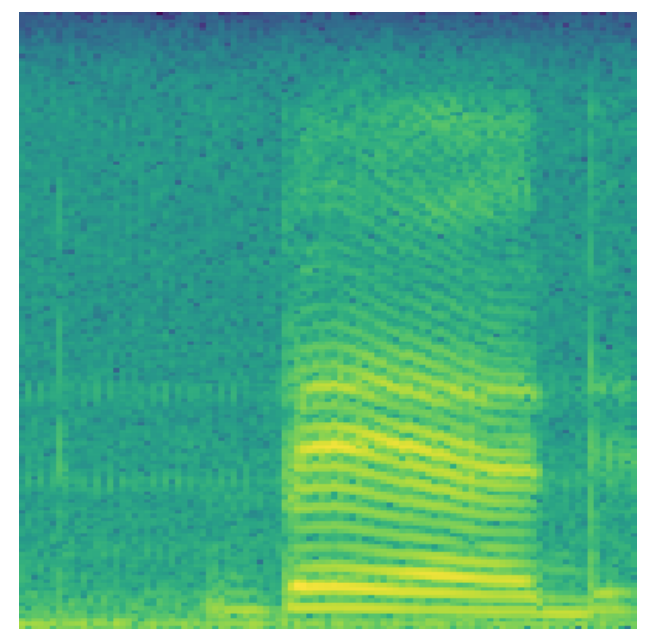
\includegraphics[width=.5\linewidth]{img/papers/image_recognition/spectrogram.png}
  \caption{}
  \label{fig:sub1}
\end{subfigure}%
\begin{subfigure}{.5\textwidth}
  \centering
  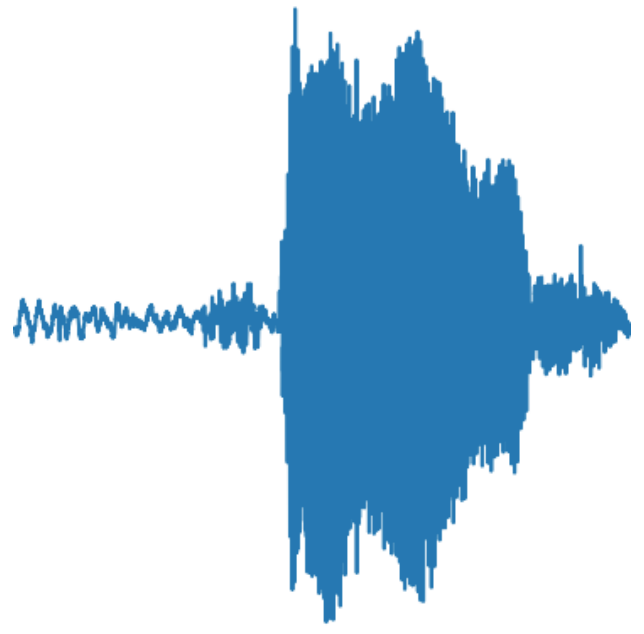
\includegraphics[width=.5\linewidth]{img/papers/image_recognition/amplitude_vs_time.png}
  \caption{}
  \label{fig:sub2}
\end{subfigure}
\caption{A comparison of the spectrogram (a) and the
amplitude-vs.-time plot (b) for the same audio recording of
a person saying the word “bed”.}
\label{fig:spectrogram_vs_time_plot}
\end{figure}








\subsection{Previous work}

This section contains the most prominent approaches to the KWS task which have been successfully applied in the past and serve as baseline models or inspirations for the proposed model in this thesis. 




Different approaches to keyword spotting like:

\begin{itemize}
	\item Deep Neural Networks (DNNs)
	\item Convolutional Neural Networks (CNNs)
	\item (Keyword/Filler) Hiddem Markov Models (HMMs)
\end{itemize}



\begin{enumerate}
	\item Problem
	\item Background (literature overview)
	\item Research Question, Hypotheses, intro to experiment
\end{enumerate}


\subsubsection{Raw waveform-based audio classification using sample-level CNN architectures}

\begin{itemize}
	\item Raw waveform-based audio classification using sample-level CNN architectures \cite{lee2017raw}
\end{itemize}


\subsubsection{Transferable deep features for keyword spotting}


\begin{itemize}
	\item Transferable deep features for keyword spotting \cite{retsinas2018transferable}
\end{itemize}

\subsubsection{Imagenet: A large-scale hierarchical image database}

\begin{itemize}
	\item Imagenet: A large-scale hierarchical image database \cite{deng2009imagenet}
\end{itemize}


\subsubsection{Imagenet classification with deep convolutional neural networks}

\begin{itemize}
	\item Imagenet classification with deep convolutional neural networks \cite{krizhevsky2012imagenet}
\end{itemize}

\subsubsection{Speech Recognition: Keyword Spotting Through Image Recognition.}

The authors of the paper "Speech Recognition: Keyword Spotting Through Image Recognition" \cite{gouda2018speech} transformed the KWS task which incoporates audio data into the domain of image classification. They used the Speech Commands Dataset \cite{warden2018speech} which contains spoken words of the length of one second in order to train and evalutate their model. According to \cite{warden2018speech}, the Speech Commands Dataset V2 \cite{scd_v2} comprises one-second audio clips which were sampled at 16KHz and containing ten words, namely "Yes", "No", "Up", "Down", "Left", "Right", "On", "Off", "Stop", and "Go", and have one additional special label for "Unknown Word", and another for "Silence" (no speech detected). A vector representation of these one-second audio clips would therefore be of the form  $\mathbb{R}^{16000}$.\\

The authors used three different models, namely:

\begin{itemize}
	\item A Low Latency Convolutional Neural Network which is designed to reduce its memory footprint by limiting the number of model parameters. This model is similar to the model called "cnn-one-fstride4" which is used in \cite{sainath2015convolutional} but differs in terms of filter size, stride, channels, dense and params. The model has been trained using Stochastic Gradient Descent and Xavier Initialization has been used in order to initialize the model weights.
	\item The MNIST TensorFlow CNN / Basic CNN where some tweaks have been performed to the first layer in order to fix dimension mismatches. A baseline architecture is described in \cite{sainath2015convolutional} (3 module setup?).
	
		\begin{itemize}
			\item \url{https://github.com/tensorflow/docs/blob/master/site/en/tutorials/estimators/cnn.ipynb}
			\item \url{https://github.com/tensorflow/tensorflow/tree/master/tensorflow/examples/tutorials/mnist}
		\end{itemize}
		
		\item Adversarially trained CNN which is inspired by MCDNN \cite{cirecsan2012multi} and AlexNet \cite{krizhevsky2012imagenet}. One shallow CNN which has been used for prototyping and hyperparameter tuning. Dropout was counter-productive and therefore Virtual Adversarial Training was used, inspired by \cite{goodfellow2016deep}.
		
\end{itemize}

Evaluated parameters in this paper:

\begin{itemize}
	\item Adversarial Training Results and Comparison with
Vanilla CNN
	\item increase in training and validation accuracy over the first ten epochs for the low-latency convolution and VAT models: a zoomed-in version of Figure 12
	\item decrease of costs over 500 epochs for the lowlatency convolution and VAT models: a zoomed-out version of Figure 13
	\item  increase of training and validation accuracy over 500 epochs for the low-latency convolution and VAT models: a zoomed-out version of Figure 10
	\item  reduction of cost over the first ten epochs for the low-latency convolution and VAT models: a zoomed-in version of Figure 11
	\item the evolution of training cross-entropy loss (blue and green) and validation accuracy (red and orange) compared between Xavier and truncated normal initialization; Xavier converges much faster and may attain better results
	\item the evolution of training cross-entropy loss (blue and green) and validation accuracy (red and orange) compared between Adam and SGD optimization; Adam converges faster than SGD but reaches the same results
	\item  effect of the number of frequency-counting buckets on the accuracy of the low-latency convolution model. The model did not benefit from the increase in available data caused by increasing the number of buckets.
	\item effect of the spectrogram window size on the accuracy of the low-latency convolution model. There is a local optimum, as there was for stride in Figure 18.
	\item effect of added background noise on the final accuracy of the low-latency convolution model. The horizontal axis is signal-noise ratio in linear units.
	\item effect of the spectrogram window stride on the accuracy of the low-latency convolution model. For low values of stride, there is too much redundancy, while larger values result in lost information.
\end{itemize}

\textbf{Conlusion}

In this project we tackled the speech recognition problem by applying different CNN models on image data formed using log spectrograms of the audio clips. We also successfully implemented a regularization method "Virtual Adversarial Training" that achieved a maximum of 92\% validation accuracy on 20\% random sample of
the input data.\\
The significant work done in this project was the demonstration of how to convert a problem in audio recognition into the better-studied domain of image classification, where the powerful techniques of convolutional neural networks are fully developed.
We also saw, particularly in the case of the low-latency convolution model, how crucial good hyperparameter tuning is to the accuracy of the model. A great number of hyperparameters must be tuned, including the many choices that go into network architecture, and any of the hyperparameters, poorly chosen, can make or break the overall performance of the model. Another contribution was the use of adversarial training to provide a regularization effect in audio recognition; this technique improved results relative even to well-established techniques such as dropout, and therefore has promising applications in the future.







\textcolor{red}{Include summary about the approach of converting the long, one dimensional vector of audio data into a spectrograms and therefore making it a image classification problem.}

\subsubsection{Convolutional neural networks for small-footprint keyword spotting}

\begin{figure}[h]
    \centering
    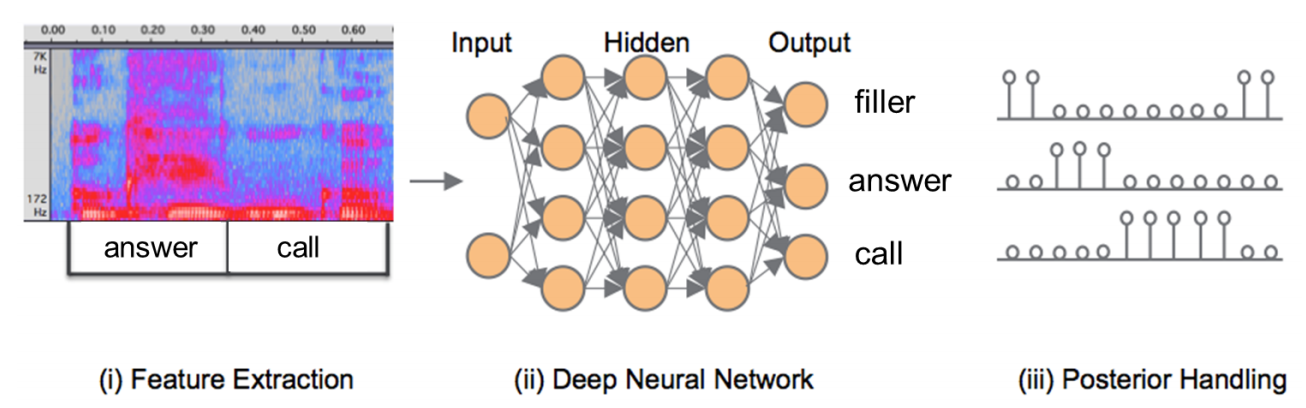
\includegraphics[width=0.75\textwidth]{img/papers/cnns_for_keyword_spotting/deep_kws_system_framework.png}
    \caption{Framework of Deep KWS system, components from
left to right: (i) Feature Extraction (ii) Deep Neural Network
(iii) Posterior Handling}
    \label{fig:deep_kws_system_frameworkl}
\end{figure}

This framework originally comes from \cite{chen2014small}. The only difference is the exchange of the DNN for a CNN.



\begin{itemize}
	\item Convolutional neural networks for small-footprint keyword spotting \cite{sainath2015convolutional}
\end{itemize}	

\textcolor{red}{Include summary about the different CNNs approaches which have been put into the 3 module framework of the below framework where the DNN has been exchanged for a CNN. How do the authors handle the long, one dimensional vector?}

\subsubsection{Small-footprint keyword spotting using deep neural networks}

\begin{itemize}
	\item Small-footprint keyword spotting using deep neural networks \cite{chen2014small}
\end{itemize}	

\textcolor{red}{Include summary about the comparison between DNNs and HMMs and the general 3 module approach here: 1. Feature extraction. 2. Deep Neural Network 3. Posterior Handling. DNNs do not need a decoding algorithm like HMMs with Viterbi which makes it low latency.}

\subsubsection{Speech Commands: A Dataset for Limited-Vocabulary Speech Recognition}


\begin{itemize}
	\item Speech Commands: A Dataset for Limited-Vocabulary Speech Recognition \cite{warden2018speech}
\end{itemize}	

\textcolor{red}{Include summary and say why the Speech Commands Dataset is a good fit for this thesis. You probably do not need a Voice-activity detection (VAD) system here.}




\textbf{Top-One Error}

\begin{quote}
The standard chosen for the TensorFlow speech commands example code is to look for the ten words "Yes", "No", "Up", "Down", "Left", "Right", "On", "Off", "Stop", and "Go", and have one additional special label for "Unknown Word", and another for "Silence" (no speech detected). The testing is then done by providing equal numbers of examples for each of the twelve categories, which means each class accounts for approximately 8.3\% of the total. The "Unknown Word" category contains words randomly samples from classes that are part of the target set. The "Silence" category has one-second clips extracted randomly from the background noise audio files.
\end{quote}

\textbf{Applications}

\begin{quote}
The TensorFlow tutorial gives a variety of baseline models, but one of the goals of the dataset is to enable the creation and comparison of a wide range of models on a lot of different platforms, and version one of has enabled some interesting applications. CMSISNN [21] covers a new optimized implementation of neural network operations for ARM microcontrollers, and uses Soeech Commands to train and evaluate the results. Listening to the World [22] demonstrates how combining the dataset and UrbanSounds [23] can improve the noise tolerance of recognition models. Did you Hear That [24] uses the dataset to test adversarial attacks on voice interfaces. Deep Residual Learning for Small Footprint Keyword Spotting \cite{tang2018deep} shows how approaches learned from ResNet can produce more efficient and accurate models. Raw Waveformbased Audio Classification \cite{lee2017raw} investigates alternatives to traditional feature extraction for speech and music models. Keyword Spotting through Image Recognition \cite{gouda2018speech} looks at the effect of virtual adversarial training on the keyword task.
\end{quote}

\textbf{Evaluation}

\begin{quote}
One of this dataset's primary goals is to enable meaningful comparisons between different models' results, so it's important to suggest some precise testing protocols. As a starting point, it's useful to specify exactly which utterances can be used for training, and which must be reserved for testing, to avoid overfitting. The dataset download includes a text file called \texttt{validation\_list.txt}, which contains a list of files that are expected to be used for validating results during training, and so can be used frequently to help adjust hyperparameters and make other model changes. The \texttt{testing\_list.txt} file contains the names of audio clips that should only be used for measuring the results of trained models, not for training or validation. The set that a file belongs to is chosen using a hash function on its name. This is to ensure that files remain in the same set across releases, even as the total number in the same set across releases, even as the total number changes, so avoid set corss-contaimination when trying old models on the more recent test data. The Python implementation of the set assignment algorithm is given in the TensorFlow tutorial code [12] that is a companion to the dataset.
\end{quote}

\textbf{Historical Evaluations}

\begin{quote}
Version 1 of the dataset \cite{scd_v1} was released August 3rd 2017, and contained 64,727 utterances from 1,881 speakers. Training the default convolution model from the TensorFlow tutorial (based on Convolutional Neural Networks for Small-footprint Keyword Spotting \cite{sainath2015convolutional}) using the V1 training data gave a Top-One score of 85.4\%, when evaluated against the test set from V1. Training the same model against version 2 of the data set \cite{scd_v2}, documented in this paper, produces a model that scores 88.2\% Top-One on the training set extracted from the V2 data. A model trained on V2 data, but evaluated against the V1 test set gives 89.7\% Top-One, which indicates that the V2 training data is responsible for a substantial improvement in accuracy over V1. The full set of results are shown in Table \ref{tab:v1_v2_results}
\end{quote}


\begin{table}[]
\center
\begin{tabular}{|c|c|c|}
\hline
Data & V1 Training & V2 Training \\ \hline
V1 Test & 85.4\% & 89.7\% \\ \hline
V2 Test & 82.7\% & 88.2\% \\ \hline
\end{tabular}
\caption{Top-One accuracy evaluations using different training data}
\label{tab:top_one_accuracy}
\end{table}




\begin{itemize}
	\item Convolutional recurrent neural networks for small-footprint keyword spotting \cite{arik2017convolutional}
	\item Honk: A PyTorch reimplementation of convolutional neural networks for keyword spotting \cite{tang2017honk}
	\item An experimental analysis of the power consumption of convolutional neural networks for keyword spotting \cite{tang2018experimental}
	\item Transfer learning for speech recognition on a budget \cite{kunze2017transfer}
	\item Learning and transferring mid-level image representations using convolutional neural networks \cite{oquab2014learning}
	\item Deep residual learning for small-footprint keyword spotting \cite{tang2018deep}
\end{itemize}


\subsection{Research Question}




\section{Method}

The method is inspired by \cite{gouda2018speech} where three different models have been evaluated on their capability to handle audio data transformed to images. One of the baseline models is the MNIST model which is also used in the Tensorflow Speech Recognition tutorial \cite{tutorial}


\begin{enumerate}
	\item methodology, types of analyses, selection of the method
\end{enumerate}


Xavier Glorot initialization \cite{glorot2010understanding}

Taken from \cite{gouda2018speech}: For an $m \times x$ dimensional matrix $M, M_{i,j}$ is assigned values selected uniformly from the distribution $[-\epsilon, \epsilon]$, where
\begin{equation} \label{eq:xavier}
\epsilon = \frac{\sqrt{6}}{\sqrt{m + n}}
\end{equation}


Xavier initialization is shown in equation \ref{eq:xavier}



\section{Set-up} \label{setup}



\subsection{Dataset} 

The TensorFlow Speech Recognition Challenge hosted by Kaggle \cite{kaggle_challenge} is using the Speech Commands Data Set v0.01 and contains 64,727 audio files and 31 class labels. The data set is publicly available \cite{scd_v1} and is explained in more detail by Warden \cite{warden2018speech}. The characteristics of the original v0.01 data set are explained as follows by Warden:

\begin{quote}
Each utterance is stored as a one-second (or less) WAVE format file, with the sample data encoded as linear 16-bit single-channel PCM values, at a 16 KHz rate. There are 2,618 speaker recorded, each with a unique eight-digit hexadecimal identifier assigned as described above. The uncompressed files take up approximately 3.8 GB on disk, and can be stored as a 2.7 GB gzip-compressed tar archive.
\end{quote}

The original class distribution of 31 words had to be reduced to 12 words to comply with the Kaggle competition guidelines, namely 10 concrete words \texttt{yes, no, up, down, left, right, on, off, stop, go} and two placeholder words \texttt{unknown, silence}. Words which do not belong to the 10 concrete words are merged into the \texttt{unknown} class label, while background noise and simple silence are merged into the \texttt{silence} class label. Provided files are further explained on the competition page \cite{kaggle_challenge} as follows:

\begin{itemize}
	\item \textbf{train.7z}: Contains a few informational files and a folder of audio files. The audio folder contains subfolders with 1 second clips of voice commands, with the folder name being the label of the audio clip. There are more labels that should be predicted. The labels you will need to predict in Test are \texttt{yes, no, up, down, left, right, on, off, stop, go}. Everything else should be considered either \texttt{unknown} or \texttt{silence}. The folder \texttt{\_background\_noise\_} contains longer clips of "silence" that you can break up and use as training input. The files contained in the training audio are not uniquely named across labels, but they are unique if you include the label folder. For example, \texttt{00f0204f\_nohash\_0.wav} is found in 14 folders, but that file is a different speech command in each folder. The files are named so the first element is the subject id of the person who gave the voice command, and the last element indicated repeated commands. Repeated commands are when the subject repeats the same word multiple times. Subject id is not provided for the test data, and you can assume that the majority of commands in the test data were from subjects not seen in train. You can expect some inconsistencies in the properties of the training data (e.g., length of the audio).
	\item \textbf{test.7z}: Contains an audio folder with 150,000+ files in the format \texttt{clip\_000044442.wav}. The task is to predict the correct label. Not all of the files are evaluated for the leaderboard score.
	\item \textbf{sample\_submission.csv}: A sample submission file in the correct format.
\end{itemize}

After merging words which do not comply with the competition guidelines, the class distribution changed from a balanced distribution to a rather unbalanced distribution towards the "unknown" label as depicted in table \ref{tab:class_distribution}


\begin{table}[h!]
\center
\begin{tabular}{|l|l|l|}
\hline
Class & Frequency & Percentage \\ \hline
unknown & '41039 & 0.634032  \\ \hline
stop & 2380 & 0.036770 \\ \hline
yes & 2377 & 0.036723  \\ \hline
up & 2375 &  0.036693\\ \hline
no & 2375 & 0.036693 \\ \hline
go & 2372 & 0.036646 \\ \hline
right & 2367 & 0.036569 \\ \hline
on & 2367 & 0.036569 \\ \hline
down & 2359 & 0.036445 \\ \hline
off & 2357 & 0.036414 \\ \hline
left & 2353 & 0.036353\\ \hline
silence & 6 & 0.000093\\ \hline
\end{tabular}
\caption{Descending class distribution of merged data set}
\label{tab:class_distribution}
\end{table}

		
		
		
		
		
		
		
		
		
		
		

\subsection{Preprocessing}

The preprocessing pipeline is described in further detail in the following subsections. The pipeline is rather simple at the moment and provides room for improvement which is described in section \ref{future_work}. The overall preprocessing approach is depicted in figure \ref{fig:preprocessing}. A Voice-activity detection (VAD) system 
has not been used based on the simple nature of the one-second audio clips.

\begin{figure}[h]
    \centering
    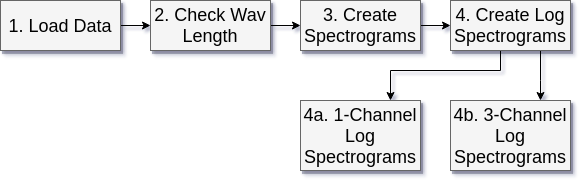
\includegraphics[width=0.8\textwidth]{img/preprocessing.png}
    \caption{Preprocessing}
    \label{fig:preprocessing}
\end{figure}


\subsubsection{Load Data}

Based on the fact that there is no index file in a common format like csv which maps data entries to labels, the approach to loading the training data involves iterating labeled folders. The training folder contains one folder for each label which then contains the actual wav files for training purposes. By iterating through the different label folders and then copying the paths of the training files, a more conventient numpy array for training purposes is used. A subset of this array is depicted in table \ref{tab:numpy_array_representation}.


\begin{table}[h!]
\center
\begin{tabular}{|l|l|}
\hline
Path & Label \\ \hline
'../data/train/audio/down/fad7a69a\_nohash\_1.wav' & 'down'  \\ \hline
'../data/train/audio/go/fa7895de\_nohash\_0.wav' & 'go'  \\ \hline
'../data/train/audio/left/fa7895de\_nohash\_0.wav'  & 'left'  \\ \hline
'../data/train/audio/no/a1c63f25\_nohash\_2.wav'   & 'no'  \\ \hline
'../data/train/audio/off/4a1e736b\_nohash\_4.wav'  & 'off'  \\ \hline
'../data/train/audio/on/4a1e736b\_nohash\_4.wav'  & 'on'  \\ \hline
'../data/train/audio/right/b71ebf79\_nohash\_0.wav'      & 'right'  \\ \hline
'../data/train/audio/\_background\_noise\_/doing\_the\_dishes.wav'  & 'silence'   \\ \hline
'../data/train/audio/stop/fa7895de\_nohash\_0.wav' & 'stop'  \\ \hline
'../data/train/audio/two/fa7895de\_nohash\_0.wav'& 'unknown'  \\ \hline
'../data/train/audio/up/4c841771\_nohash\_2.wav' & 'up'  \\ \hline
'../data/train/audio/yes/b71ebf79\_nohash\_0.wav' & 'yes'  \\ \hline
\end{tabular}
\caption{Training data - Numpy array representation}
\label{tab:numpy_array_representation}
\end{table}


The different paths were iterated and the wav files were loaded into memory by using the \texttt{scipy.io.wavfile} package. The sample rate of the wav files remains at 16000 KHz.  A reduction to a sampling rate of 8000 KHz would also be possible to reduce the used memory space for the final training set.


\subsubsection{Check Wav Length}

In order to have a consistent dataset with clips of one second length, the length of each wav file has been checked. Two approaches to guarantee one second clips have been applied:

\begin{itemize}
	\item $length < 1 \; second$: Pad the clip with constant zeros
	\item $length > 1 \; second$: Cut the clip from the beginning to the one second mark
\end{itemize}
 

\subsubsection{Create Spectrograms}

To transform audio data into images, the $\mathbb{R}^{16000}$ audio vectors have been transformed into spectrograms. The code for the transformation is given in listing \ref{code:spectrograms}.



\begin{lstlisting}[language=Python, caption=Get spectrogram code, label=code:spectrograms]
from scipy import signal
from scipy.io import wavfile
import numpy as np

def get_spectrogram(audio_path, num_channels=1):
    (sample_rate, sig) = wavfile.read(audio_path)

    if sig.size < sample_rate:
        sig = np.pad(sig, (sample_rate - sig.size, 0), mode='constant')
    else:
        sig = sig[0:sample_rate]

    # f = array of sample frequencies
    # t = array of segment times
    # Sxx = Spectrogram of x. By default, the last axis of Sxx corresponds to the segment times.
    f, t, Sxx = signal.spectrogram(sig, nperseg=256, noverlap=128)
    Sxx = (np.dstack([Sxx] * num_channels)).reshape(129, 124, -1)

    return f, t, Sxx
\end{lstlisting}

After a first inspection of the spectrograms given in figure \ref{fig:spectrograms}, it is obvious that the spectrograms do not contain as much visible features as expected. Previous research \cite{gouda2018speech} also suggested that using log spectrograms is more beneficial than using simple spectrograms. Spectrograms were reshaped into \texttt{129 x 124} dimensions which differs from the log spectrograms but does not influence the experiment in any way because solely log spectrograms were used for training purposes.


\begin{figure}[h!]
    \centering
    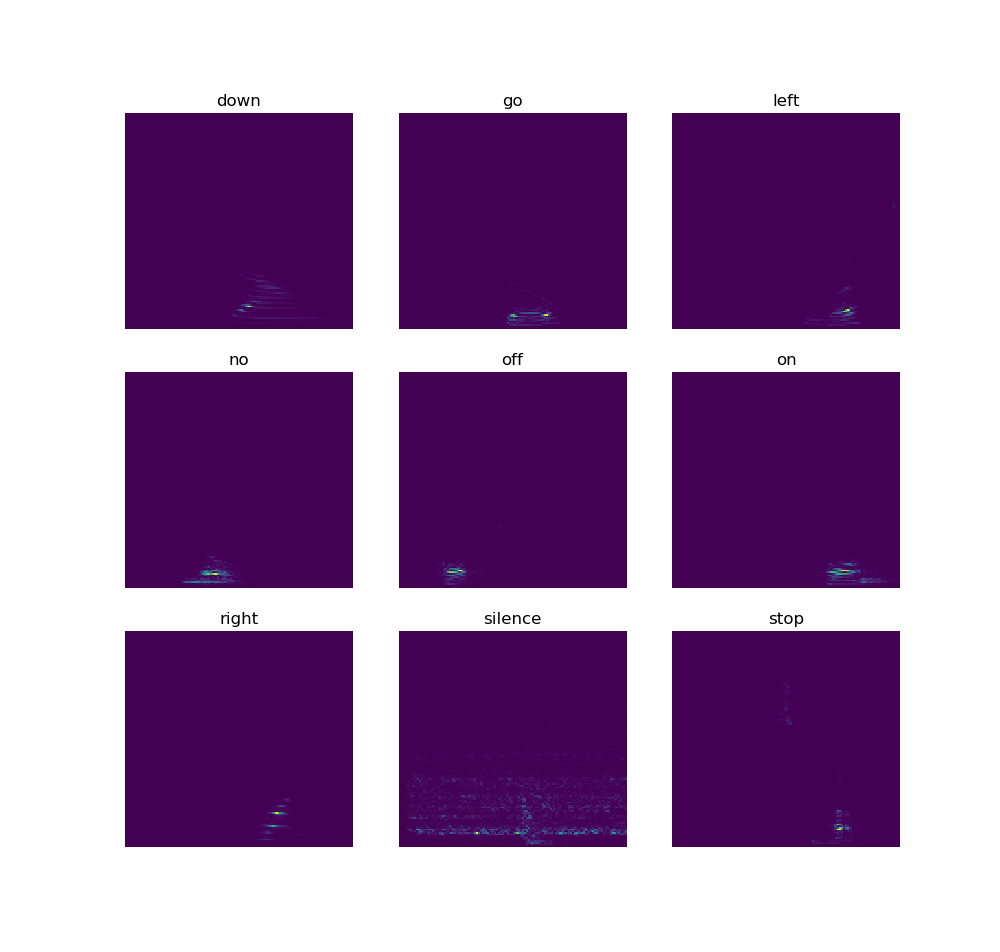
\includegraphics[width=1\textwidth]{img/9_spectrograms.png}
    \caption{Spectrogram samples of nine different classes}
    \label{fig:spectrograms}
\end{figure}



\subsubsection{Create Log Spectrograms}

In contrast to figure \ref{fig:spectrograms}, the code depicted in listing \ref{code:log_spectrograms} produces log spectrograms which contain more visual features as seen in figure \ref{fig:log_spectrograms} which should be beneficial for the model training. One potential problem however is shown in figure \ref{fig:log_spectrograms} at the "silence" class. The padding with zeroes presents itself with a dark bar at the beginning which might introduce more noise into the dataset. Nevertheless, for this experiment this potential problem is ignored and could be tackled in future work. Log spectrograms were reshaped into \texttt{99 x 161} dimensions.

\begin{lstlisting}[language=Python, caption=Get log spectrogram code, label=code:log_spectrograms]
from scipy import signal
from scipy.io import wavfile
import numpy as np

def get_log_spectrogram(audio_path, window_size=20, step_size=10, eps=1e-10, num_channels=1):
    (sample_rate, sig) = wavfile.read(audio_path)

    if sig.size < 16000:
        sig = np.pad(sig, (sample_rate - sig.size, 0), mode='constant')
    else:
        sig = sig[0:sample_rate]

    nperseg = int(round(window_size * sample_rate / 1e3))
    noverlap = int(round(step_size * sample_rate / 1e3))

    # f = array of sample frequencies
    # t = array of segment times
    # Sxx = Spectrogram of x. By default, the last axis of Sxx corresponds to the segment times.
    f, t, Sxx = signal.spectrogram(sig,
                                   fs=sample_rate,
                                   window='hann',
                                   nperseg=nperseg,
                                   noverlap=noverlap,
                                   detrend=False)
    log_spectrogram = np.log(Sxx.T.astype(np.float32) + eps)
    log_spectrogram = (np.dstack([log_spectrogram] * num_channels)).reshape(99, 161, -1)  

    return f, t, log_spectrogram
\end{lstlisting}


\begin{figure}[h!]
\centering
\begin{subfigure}{.34\textwidth}
  \centering
  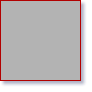
\includegraphics[width=0.5\linewidth]{img/grayscale.png}
  \caption{1-channel log spectrogram}
  \label{fig:sub1}
\end{subfigure}%
\begin{subfigure}{.34\textwidth}
  \centering
  
\includegraphics[width=0.5\linewidth]{img/rgb.png}
  \caption{3-channel RGB image}
  \label{fig:sub2}
\end{subfigure}
\par\bigskip
\begin{subfigure}{.5\textwidth}
  \centering
  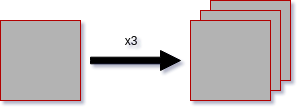
\includegraphics[width=1\linewidth]{img/grayscale_multiply.png}
  \caption{Duplication of 1-channel log spectrogram}
  \label{fig:sub2}
\end{subfigure}
\caption{Conversion between 1-channel and 3-channel log spectrograms}
\label{fig:channel_conversion}
\end{figure}


\begin{figure}[h!]
    \centering
    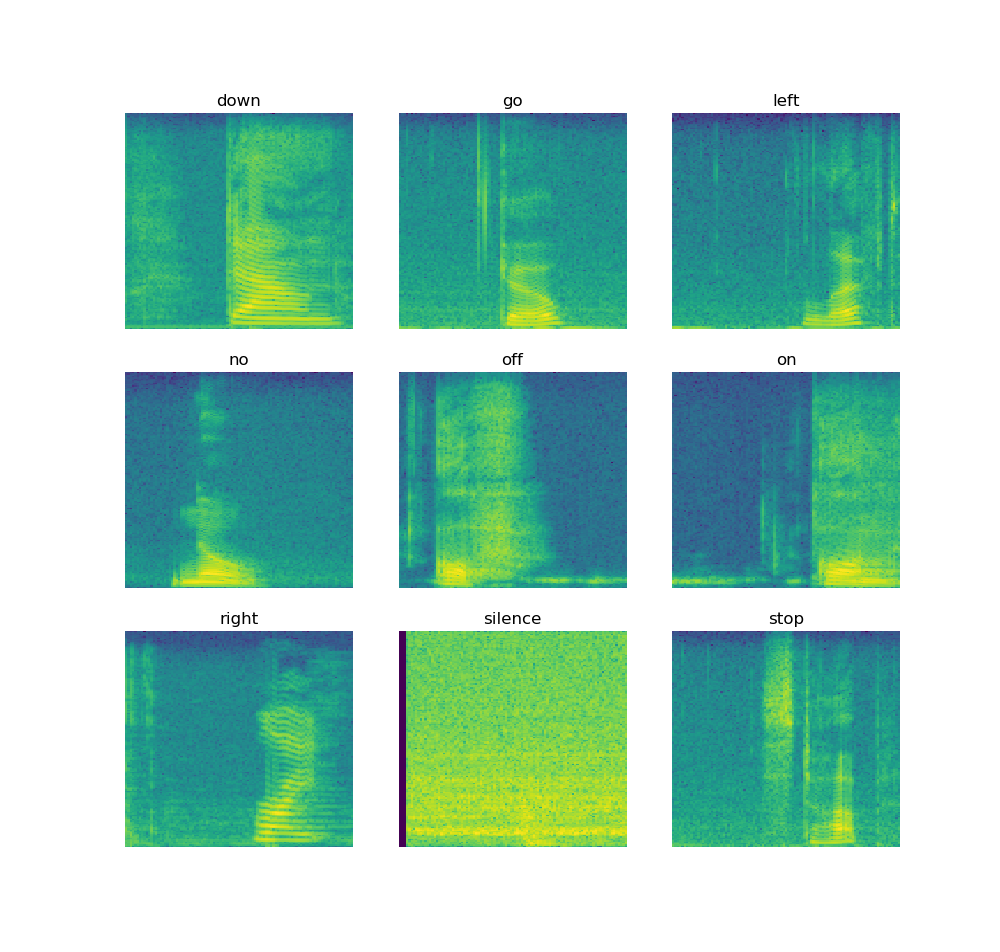
\includegraphics[width=1\textwidth]{img/9_log_spectrograms.png}
    \caption{Log spectrogram samples of nine different classes}
    \label{fig:log_spectrograms}
\end{figure}

A distinction between 1- and 3-channel log spectrograms has been made because this project uses pre-trained CNN models which are trained on ImageNet data. ImageNet data is in its core based on 3-dimensional RGB data/images while (log) spectrograms are 1-dimensional images and are only depicted in green colors in figure \ref{fig:log_spectrograms} based on the settings in the \texttt{matplotlib} package which shows grayscale images in a green spectrum. A quick fix to this problem is the duplication of the 1-dimensional spectrogram data and therefore mimicking 3-dimensional RGB data by having the grayscale data copied over three channels as depicted in figure \ref{fig:channel_conversion}.

\newpage

\subsection{Parameters}


All models used Rectified Linear Unit as depicted in figure \ref{fig:relu} as their activation function due to its success in the domain of image classification \cite{dahl2013improving}. However, Softmax is applied as the final activation function in all output layers in order get proper probabiliy scores.

\newpage


\begin{figure}[h!]
    \centering
    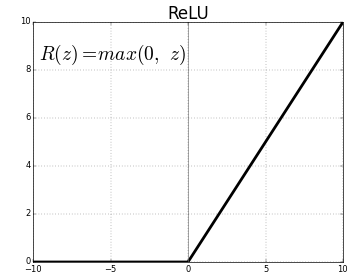
\includegraphics[width=0.5\textwidth]{img/relu.png}
    \caption{Rectified Linear Unit as activation function}
    \label{fig:relu}
\end{figure}

Throughout all architectures Dropout has been used \cite{srivastava2014dropout} with a value of $0.2$ as a regularization technique as depicted in figure \ref{fig:dropout} and as proposed in \cite{dahl2013improving}.


\begin{figure}[h!]
    \centering
    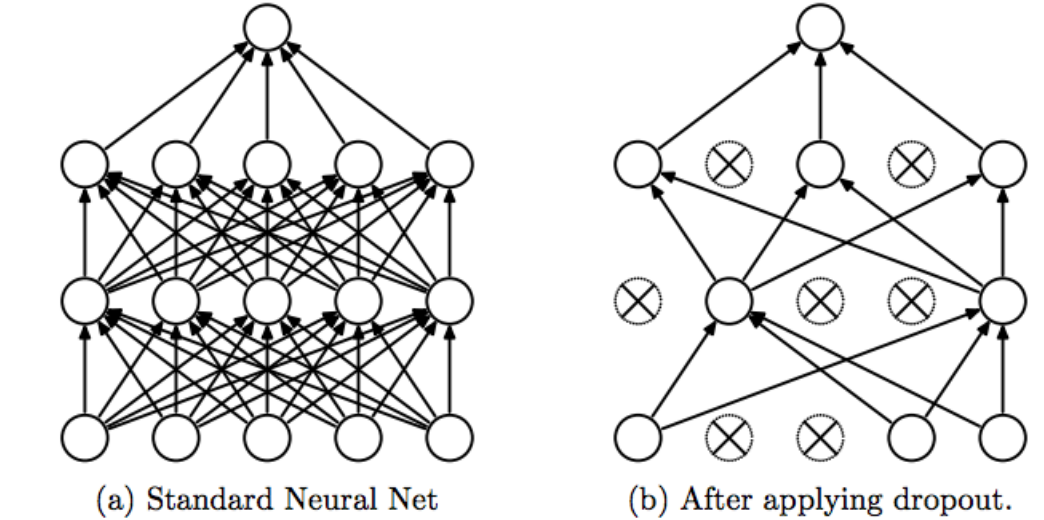
\includegraphics[width=0.65\textwidth]{img/dropout.png}
    \caption{Dropout as generalization technique}
    \label{fig:dropout}
\end{figure}

Batch normalization as depicted in figure \ref{fig:dropout} and proposed in \cite{ioffe2015batch} has been applied to all architectures due to the memory space consumption of the training set and the need to use a batch size of 32. Batch normalization showed good results in boosting the overall training process of feedforward neural networks with fewer training steps, acts as a additional regularization technique and reduces internal covariate shift by normalizing each batch respectively. 


\begin{figure}[h!]
    \centering
    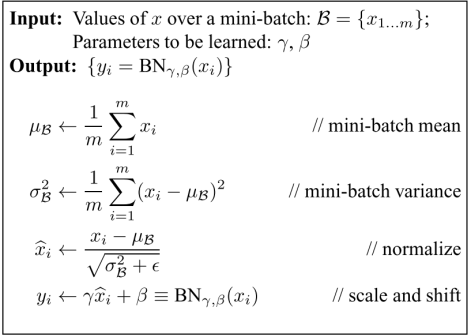
\includegraphics[width=0.65\textwidth]{img/bn.png}
    \caption{Batch normalization to speed up training and reducing internal covariate shift}
    \label{fig:dropout}
\end{figure}

Adam \cite{kingma2014adam} has been used as the main optimization technique for all models with a learning rate of $0.001$ while the training set has been split up into a 80\% training and 20\% validation set. An overview of the parameters is shown in table \ref{tab:overall_parameters}


\begin{table}[h!]
\center
\begin{tabular}{|l|l|}
\hline
\textbf{Parameter} & \textbf{Value}  \\ \hline
Dropout & 0.2 \\ \hline
Optimization & Adam\\ \hline
Loss & Categorical Crossentropy \\ \hline
Training/validation ratio & 80:20\\ \hline
Epochs & 10 \\ \hline
Batch size & 32 \\ \hline
Activation & ReLU \\ \hline
\end{tabular}
\caption{Overall parameters}
\label{tab:overall_parameters}
\end{table}

\newpage


\subsection{Models} \label{models}

The choice of models can be divided into the following groups: \textbf{Baseline} and \textbf{CNN models with pre-trained ImageNet weights}. Table \ref{tab:model_complexity} shows an overview of the evaluated models in this project with the complexity of each model based on its amount of trainable parameters.\\
MNIST and the Lightweight CNN model are used as a baseline because they showed good performance in previous work when applied to spectrograms. The other models, namely VGG16, Inception V3 and ResNet50 were used because they each won the ImageNet Large Scale Visual Recognition Challenge (ILSVRC) in their respective years and differ in their architecture. The baseline models were initialized with Xavier initialization and their performances were not evaluated with ImageNet weight initialization.\\


\begin{table}[h!]
\center
\begin{tabular}{|l|l|l|l|}
\hline
\textbf{Model} & \textbf{Total params} & \textbf{Trainable params} & \textbf{Non-trainable params} \\ \hline
Lightweight CNN & 723,968 & 723,454 & 514 \\ \hline
VGG16  		& 23,676,748   & 23,659,340        & 17,408 \\ \hline	
Inception V3	& 29,185,836   & 29,137,068  	   & 48,768	 \\ \hline
MNIST			& 55,038,988   & 54,929,868   	   & 109,120  \\ \hline
ResNet50  	& 75,182,988   & 75,029,516 	   & 153,472 \\ \hline	
\end{tabular}
\caption{Model complexity ordered by amount of parameters}
\label{tab:model_complexity}
\end{table}

Each model has been trained over 10 epochs with either Xavier Glorot initialization while the CNN models have also been using pre-trained ImageNet weights while all layers remained trainable which is against traditional transfer learning techniques where a certain amount of layers are not trainable any more (freezing layers). After 10 epochs the final accuracy has been evaluated in order to see if pre-trained ImageNet weights would give a boost to the convergence rate. Another evaluation has been made after the first epoch with regards to accuracy to see if pre-trained ImageNet weights would give a higher start accuracy based on the already learned image features from another domain than the provided spectrograms, namely general images in the ImageNet dataset.\\



The following sections include descriptions of the architecture and special characteristics of each model. 



\subsubsection{Baseline models}


\noindent\textbf{MNIST}\\

The chosen architecture of the so called "MNIST" model is burrowed from the TensorFlow repository \cite{mnist_code} and showed an accuracy of 98\% on the task for grayscale digit recognition \cite{deng2012mnist}. In order to guarantee consistent comparison conditions, batch normalization layers have been added. The MNIST architecture therefore looks as follows:

\begin{enumerate}
	\item 2D Convolutional layer with 32 features, kernel size of $5 \times 5$ and ReLU activation function.
	\item MaxPooling layer with a pool size of $2 \times 2$
	\item Batch normalization layer with $momentum=0.99, \epsilon=0.001$
	\item 2D Convolutional layer with 64 features, kernel size of $3 \times 3$ and ReLU activation function.
	\item MaxPooling layer with a pool size of $2 \times 2$
	\item Dropout layer with $p = 0.2$
	\item Batch normalization layer with $momentum=0.99, \epsilon=0.001$
	\item Dense layer with 1024 neurons and ReLU activation
	\item Dropout layer with $p = 0.2$
	\item Batch normalization layer with $momentum=0.99, \epsilon=0.001$
	\item Dense layer with 12 neurons (number of classes) and Softmax
\end{enumerate}



\noindent\textbf{Lightweight CNN}\\

The "Lightweight CNN" has been burrowed from the Kaggle competition in order to have another baseline model which is known to perform well with spectrograms \footnote{\url{https://www.kaggle.com/alphasis/light-weight-cnn-lb-0-74}}. The main architecture looks as follows:


\begin{enumerate}
		\item Batch normalization layer with $momentum=0.99, \epsilon=0.001$
		\item 2x 2D Convolutional layer with 8 features, kernel size of $2 \times 2$ and ReLU activation function.
		\item MaxPooling layer with a pool size of $2 \times 2$
		\item Dropout layer with $p = 0.2$
		\item 2x 2D Convolutional layer with 16 features, kernel size of $3 \times 3$ and ReLU activation function.
		\item MaxPooling layer with a pool size of $2 \times 2$
		\item Dropout layer with $p = 0.2$
		2D Convolutional layer with 32 features, kernel size of $3 \times 3$ and ReLU activation function.
			\item MaxPooling layer with a pool size of $2 \times 2$
			\item Dropout layer with $p = 0.2$
		\item Batch normalization layer with $momentum=0.99, \epsilon=0.001$
			\item Dense layer with 128 neurons and ReLU activation function
		\item Batch normalization layer with $momentum=0.99, \epsilon=0.001$
		\item Dense layer with 128 neurons and ReLU activation function
		\item Dense layer with 12 neurons (number of classes) and Softmax
		
\end{enumerate}


\subsubsection{CNN models} \label{cnn_models}

The top layers of each CNN model have been removed in order to take other input tensors than the usual ones found in the ImageNet database which are \texttt{224x224} pixels to fit the log spectrogram dimensions. The here called "standard top layer configuration" has been stacked on top of every CNN model in order to have a consistent configuration and to work with log spectrograms. The standard top layer configuration looks as follows:

\begin{enumerate}
	\item Dropout layer with $p = 0.2$
	\item Batch normalization layer with $momentum=0.99, \epsilon=0.001$
	\item Dense layer with 1024 neurons and ReLU activation function
	\item Batch normalization layer with $momentum=0.99, \epsilon=0.001$
	\item Dense layer with 1024 neurons and ReLU activation
	\item Dense layer with 12 neurons (number of classes) and Softmax activation function
\end{enumerate}

CNN models which originally do not use batch normalization therefore get this feature on top in order to make the models more comparable to each other.\\


\noindent\textbf{VGG16}\\

The VGG architecture has been proposed in 2014 and incorporates increasing depth using an architecture with very small $(3 \times 3)$ convolutional filters and a depth of 16 to 19 weight layers \cite{simonyan2014very}. The main VGG architecture \footnote{\url{https://neurohive.io/en/popular-networks/vgg16/}} is depicted in figure \ref{fig:vgg16_architecture} and also won the ImageNet Challenge in 2014.

\begin{figure}[h!]
    \centering
    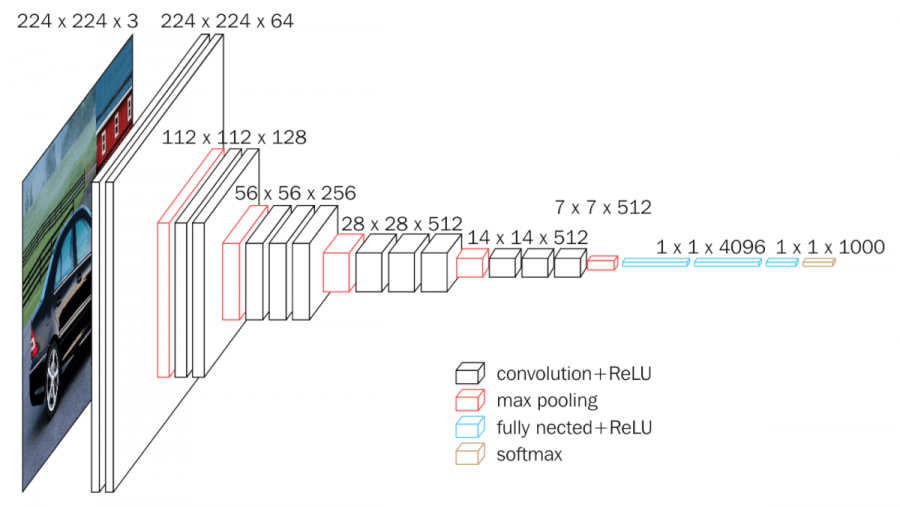
\includegraphics[width=1\textwidth]{img/vgg16_architecture.png}
    \caption[VGG16 architecture]{VGG16 architecture}
    \label{fig:vgg16_architecture}
\end{figure}

Because VGG16 is such a commonly used CNN model in the domain of image classification and used in prior work with keyword spotting, it is also used in this project as the default CNN. Furthermore, Keras also kindly provides the Python code and the pre-trained ImageNet weights for this model \cite{vgg16_impl}.\\




\noindent\textbf{Inception V3}\\

The Inception V3 architecture is the winner of the ImageNet Challenge of 2015 and outperformed the VGG architecture \cite{szegedy2016rethinking}. Its main architecture is depicted in figure \ref{fig:inception}. The architecture is 42 layers deep while the computation cost is only about 2.5 higher than that of GoogLeNet, and much more efficient than that of VGG  \footnote{\url{https://medium.com/@sh.tsang/review-inception-v3-1st-runner-up-image-classification\\-in-ilsvrc-2015-17915421f77c}}. This efficiency is accomplished by using an efficient grid size reduction compared to a greedy max pooling operation in the convolutional layers like VGG16.

\begin{figure}[h!]
    \centering
    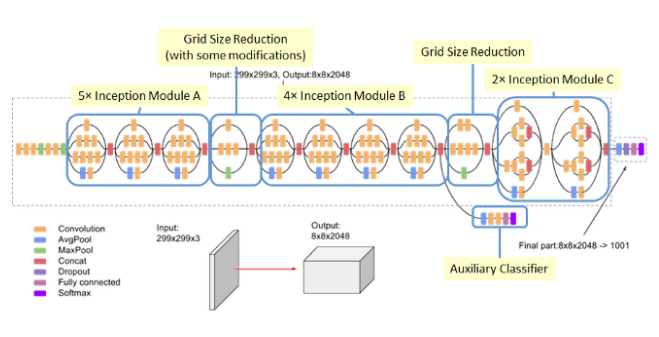
\includegraphics[width=1\textwidth]{img/inception.png}
    \caption{Inception-v3 Architecture (Batch Norm and ReLU are used after Conv)}
    \label{fig:inception}
\end{figure}


In order to draw good conlusions with regards to the benefits of the ImageNet initialization strategy while being architecture-agnostic at the same time, Inception V3 differs from the VGG16 model sufficiently to use it as the second CNN model. Furthermore, Keras also kindly provides the Python code and the pre-trained ImageNet weights for this model \cite{inception}.\\
\newpage

\noindent\textbf{ResNet50}\\

Deep residual networks outperformed the VGG architecture in the task of image classification by being eight times deeper than VGG nets but still having lower complexity \cite{he2016deep}. So called "Skip connections" which are the building blocks of residual learning can be used to skip the training of a few layers as depicted in figure \ref{fig:skip_connection}.


\begin{figure}[h!]
    \centering
    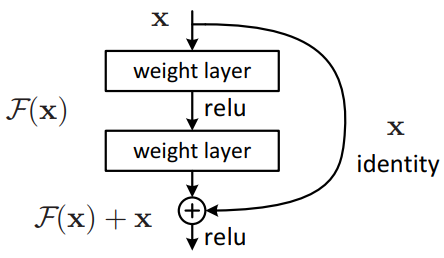
\includegraphics[width=0.5\textwidth]{img/skip_connections.png}
    \caption{Residual learning: a building block.}
    \label{fig:skip_connection}
\end{figure}

Deep residual learning has also been applied to the domain of small-footprint keyword spotting and outperformed classical CNN architectures \cite{tang2018deep} which makes it a good fit for this project. Keras standard "ResNet50" model \cite{resnet50} has been used with the standard top layer configuration.




\section{Experiments}

The main factors in this experiment are the accuracy and loss metrics for both the training and validation set after (i) the first epoch and (ii) after the last epoch which is set to 10 for all models.\\

\begin{enumerate}
	\item[i] The inspection of the first epoch should show if there are higher accuracy/lower loss values at the beginning of the training process depending on which initialization strategy was chosen
	\item[ii] The inspection of the last epoch should show if there are higher accuracy/lower loss values at the end of the training process and if the convergence rate is higher towards a maximum depending on which initialization strategy was chosen
\end{enumerate}

The first part of the experiment focuses on the baseline models, namely MNIST and the lightweight CNN. These models are not initialized with pre-trained ImageNet weights but solely with Xavier Glorot initialization. The baseline models serve as a starting point with regards to accuracy and loss values.\\

The second part of the experiment focuses on the CNN models for which pre-trained ImageNet weights exist. The models are evaluated with regards to point (i) and (ii) with Xavier Glorot Initialization and with pre-trained ImageNet weights.\\

The results of the first part are used for evaluationg the overall performance of the CNN models while the second answers the main research question if pre-trained ImageNet weights are beneficial when it comes to the task of speech recognition on spectrograms. All other parameters which are descibed in section \ref{models} remain the same.




\section{Analysis and Results}

The following sections contain the results of the previously described experimental setup.

\subsection{Baseline}

According to table \ref{tab:one_epoch_baseline_results_xavier}, the initial values of the MNIST and lightweight CNN model do not differ significantly while the lightweight CNN performs slighty better on both the training and validation set. The training accuracy is $\approx 70\%$ for both models at the beginning and should serve as the baseline accuracy value for later comparison.

\begin{table}[h!]
\center
\begin{tabular}{|l|l|l|l|l|l|}
\hline
\textbf{Model} & \textbf{Train Acc} & \textbf{Train Loss} & \textbf{Val Acc} & \textbf{Val Loss}\\ \hline
MNIST		  & 0.7005  & 1.0187   & 0.7662 & 0.7237 \\ \hline
Lightweight CNN    & 0.7150  & 0.9276  & 0.8114  &	0.5540 \\ \hline
\end{tabular}
\caption{Baseline results after one epoch with Xavier Glorot initialization}
\label{tab:one_epoch_baseline_results_xavier}
\end{table}

During the training process a clear convergence towards a maximum is evident in both the MNIST and lightweight CNN model as depicted in figure \ref{fig:mnist_ten_epochs} and \ref{fig:lightweight_cnn_ten_epochs} respectively. 


\begin{figure}[h!]
\centering
\begin{subfigure}{.5\textwidth}
  \centering
  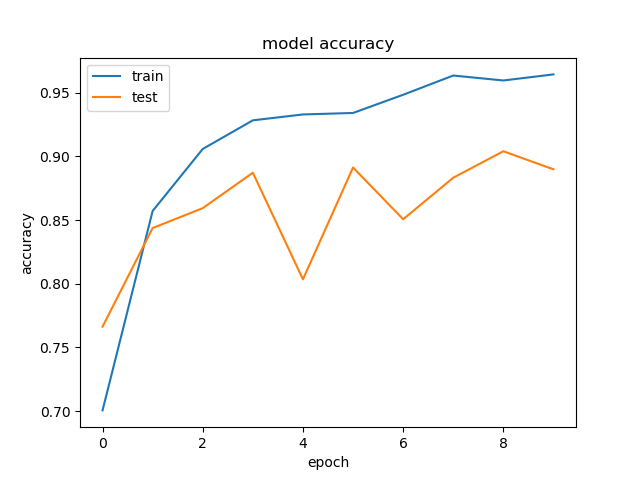
\includegraphics[width=1.2\linewidth]{img/baseline_models/mnist_acc.png}
  \caption{Accuracy}
  \label{fig:sub1}
\end{subfigure}%
\begin{subfigure}{.5\textwidth}
  \centering
  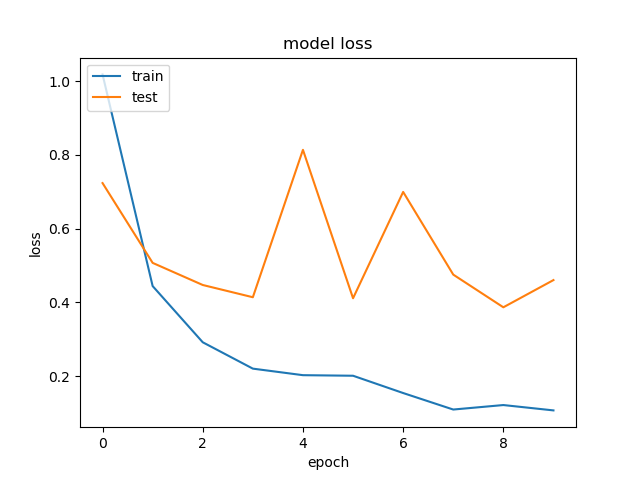
\includegraphics[width=1.2\linewidth]{img/baseline_models/mnist_loss.png}
  \caption{Loss}
  \label{fig:sub2}
\end{subfigure}
\caption{Accuracy and loss after 10 epochs for the MNIST model with Xavier Glorot initialization}
\label{fig:mnist_ten_epochs}
\end{figure}


\begin{figure}[h!]
\centering
\begin{subfigure}{.5\textwidth}
  \centering
  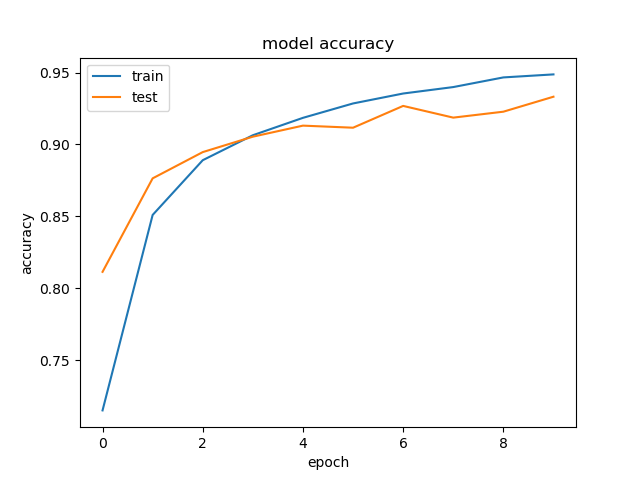
\includegraphics[width=1.2\linewidth]{img/baseline_models/leightweight_cnn_acc.png}
  \caption{Accuracy}
  \label{fig:sub1}
\end{subfigure}%
\begin{subfigure}{.5\textwidth}
  \centering
  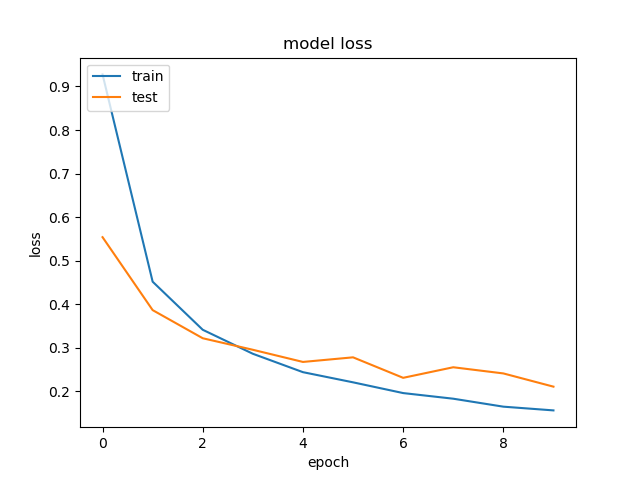
\includegraphics[width=1.2\linewidth]{img/baseline_models/leightweight_cnn_loss.png}
  \caption{Loss}
  \label{fig:sub2}
\end{subfigure}
\caption{Accuracy and loss after 10 epochs for the Lightweight CNN model with Xavier Glorot initialization}
\label{fig:lightweight_cnn_ten_epochs}
\end{figure}


\begin{table}[h!]
\center
\begin{tabular}{|l|l|l|l|l|l|}
\hline
\textbf{Model} & \textbf{Train Acc} & \textbf{Train Loss} & \textbf{Val Acc} & \textbf{Val Loss} & \textbf{Time (sec)}\\ \hline
MNIST		    & 0.9595 		 & 0.1213      & 0.9039		  & 0.3866	 &	1064.72\\ \hline
Lightweight CNN    & 0.9487   	 & 0.1564 	   & 0.9332		  &	0.2109	 &  532.73 \\ \hline
\end{tabular}
\caption{Final baseline results with Xavier Glorot initialization}
\label{tab:final_baseline_results_xavier}
\end{table}

The final training accuracies of both models also do not differ significantly according to table \ref{tab:final_baseline_results_xavier} and are $\approx 95\%$.

\newpage

\subsection{CNNs}

The following subsections contain the results of the three different CNN models, namely VGG16, Inception V3 and ResNet50 with the Xavier Glorot initialization and the pre-trained ImageNet weights initialization.


\subsubsection{Xavier initialization}

All three CNN models lay in the same range of initial accuracy values which is between 65\% and 70\% but is still below the initial values of the baseline models. Resnet performed the best in the initial run of all three models with about a 4\% higher accuracy than VGG16 and Inception V3.



\begin{table}[h!]
\center
\begin{tabular}{|l|l|l|l|l|l|}
\hline
\textbf{Model} & \textbf{Train Acc} & \textbf{Train Loss} & \textbf{Val Acc} & \textbf{Val Loss}\\ \hline
Inception V3 & 0.6539 	& 1.4176 	 &  0.6778	 & 1.1090\\ \hline
VGG16  		& 0.6519   	& 1.3202     &  0.6906	 &	1.3379\\ \hline
ResNet50  	& 0.6916  	& 1.2478 	 &  0.6351	 &	5.7467\\ \hline
\end{tabular}
\caption{CNN results after one epoch with Xavier Glorot initialization}
\label{tab:one_epoch_cnn_results_xavier}
\end{table}

When it comes to the final accuracy values as depicted in table \ref{tab:final_cnn_results_xavier}, only Inception V3 performed worse than the baseline models while ResNet performed equally well as MNIST. VGG16 reached the highest training accuracy with about 97\%. So, VGG16 started with the lowest initial training accuracy but achieved the highest training accuracy at the end of 10 epochs from the three CNN models.\\
According to figure \ref{fig:inception_v3_ten_epochs_xavier}, Inception V3 started with some heavy fluctuation in the beginning until the third epoch and then converged towards a maximum with regards to accuracy. 

\begin{table}[h!]
\center
\begin{tabular}{|l|l|l|l|l|l|}
\hline
\textbf{Model} & \textbf{Train Acc} & \textbf{Train Loss} & \textbf{Val Acc} & \textbf{Val Loss} & \textbf{Time (sec)}\\ \hline
Inception V3	& 0.9338 & 0.2238  & 0.9427	& 0.1868 &	2332.23\\ \hline
VGG16  		& 0.9723   & 0.0900   & 0.9583	&	0.2011 &  2530.47\\ \hline
ResNet50  	& 0.9548  & 0.1421 	& 0.9445 &	0.1873	 &  3807.93\\ \hline
\end{tabular}
\caption{Final CNN results with with Xavier Glorot initialization}
\label{tab:final_cnn_results_xavier}
\end{table}


\newpage

\begin{figure}[h!]
\centering
\begin{subfigure}{.5\textwidth}
  \centering
  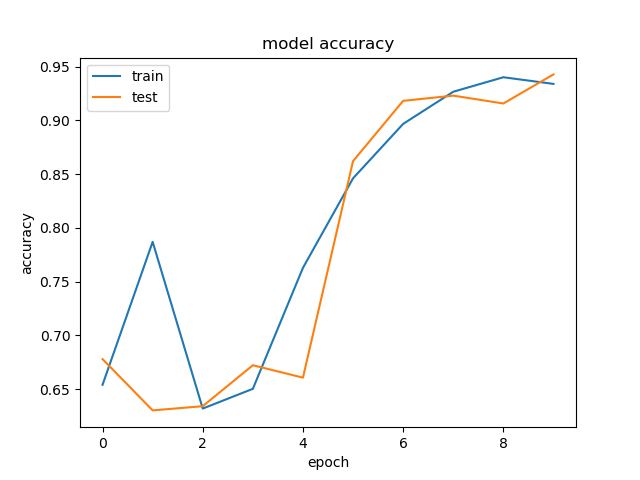
\includegraphics[width=1.2\linewidth]{img/from_scratch_models/Inceptionv3_acc.png}
  \caption{Accuracy}
  \label{fig:sub1}
\end{subfigure}%
\begin{subfigure}{.5\textwidth}
  \centering
  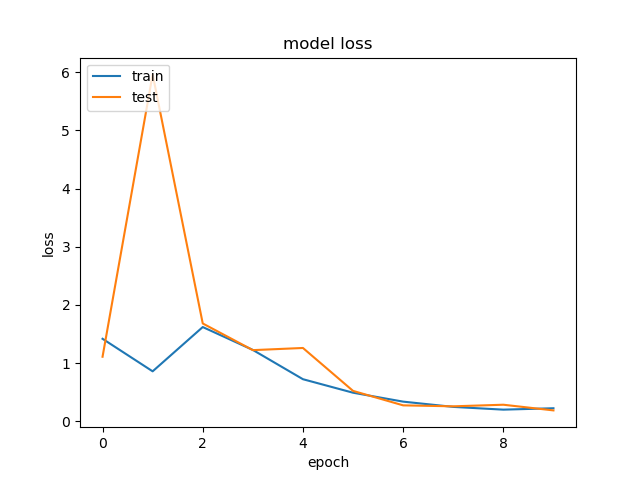
\includegraphics[width=1.2\linewidth]{img/from_scratch_models/Inceptionv3_loss.png}
  \caption{Loss}
  \label{fig:sub2}
\end{subfigure}
\caption{Accuracy and loss after 10 epochs for the Inception V3 model with Xavier Glorot initialization}
\label{fig:inception_v3_ten_epochs_xavier}
\end{figure}

VGG16 and ResNet converged more smoothly in contrast to Inception V3 when it comes to accuracy values and did not encounter fluctuation as Inception V3 as depicted in figure \ref{fig:vgg16_ten_epochs_xavier} and \ref{fig:resnet50_ten_epochs_xavier} respectively.


\begin{figure}[h!]
\centering
\begin{subfigure}{.5\textwidth}
  \centering
  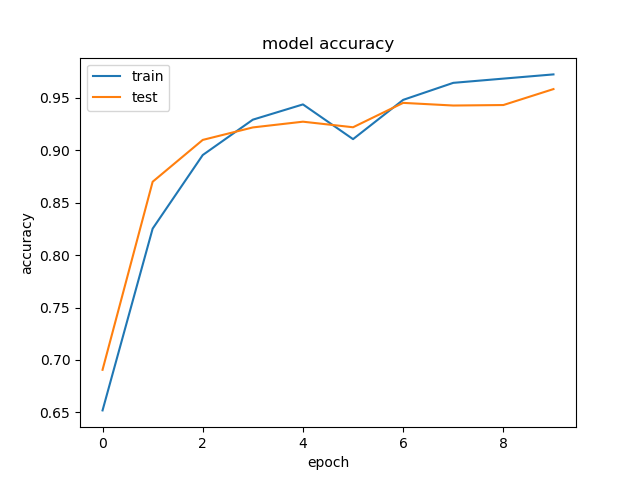
\includegraphics[width=1.2\linewidth]{img/from_scratch_models/vgg16_acc.png}
  \caption{Accuracy}
  \label{fig:sub1}
\end{subfigure}%
\begin{subfigure}{.5\textwidth}
  \centering
  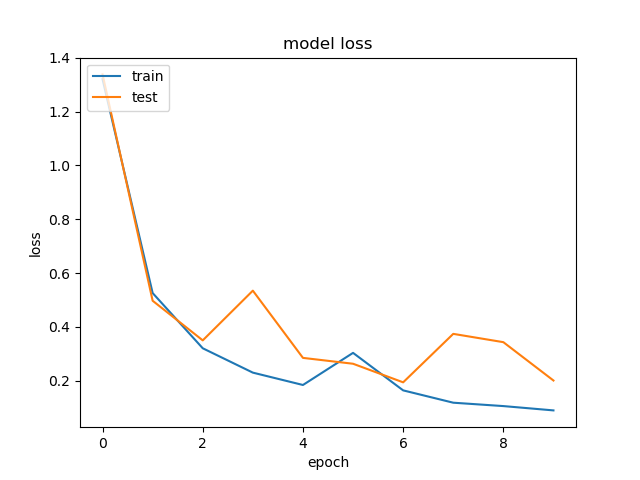
\includegraphics[width=1.2\linewidth]{img/from_scratch_models/vgg16_loss.png}
  \caption{Loss}
  \label{fig:sub2}
\end{subfigure}
\caption{Accuracy and loss after 10 epochs for the VGG16 model with Xavier Glorot initialization}
\label{fig:vgg16_ten_epochs_xavier}
\end{figure}

\begin{figure}[h!]
\centering
\begin{subfigure}{.5\textwidth}
  \centering
  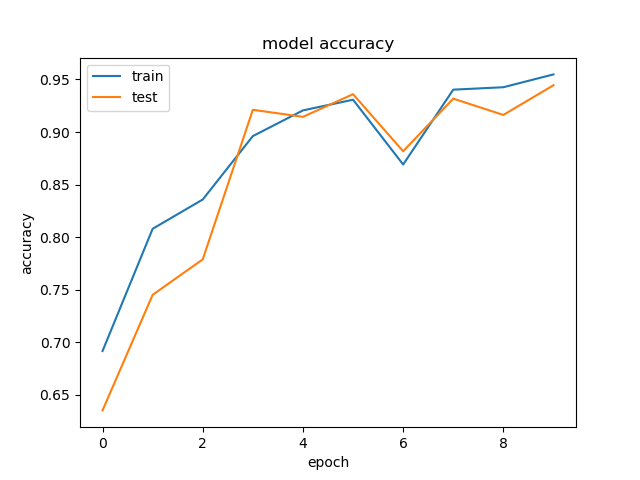
\includegraphics[width=1.2\linewidth]{img/from_scratch_models/ResNet50_acc.png}
  \caption{Accuracy}
  \label{fig:sub1}
\end{subfigure}%
\begin{subfigure}{.5\textwidth}
  \centering
  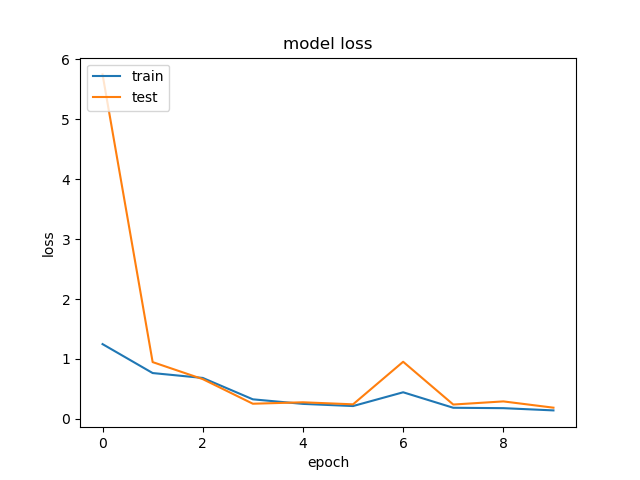
\includegraphics[width=1.2\linewidth]{img/from_scratch_models/ResNet50_loss.png}
  \caption{Loss}
  \label{fig:sub2}
\end{subfigure}
\caption{Accuracy and loss after 10 epochs for the ResNet50 model with Xavier Glorot initialization}
\label{fig:resnet50_ten_epochs_xavier}
\end{figure}







\subsubsection{Imagenet weight initialization}

The initial values of all three CNN models initialized with the pre-trained ImageNet weights lay around 62\% and 63\% depicted in table \ref{tab:one_epoch_cnn_results_imagenet}. These values are worse than the baseline model values shown in table \ref{tab:one_epoch_baseline_results_xavier} and the CNN models which are initialized with Xavier Glorot initialization shown in table \ref{tab:one_epoch_cnn_results_xavier}.


\begin{table}[h!]
\center
\begin{tabular}{|l|l|l|l|l|l|}
\hline
\textbf{Model} & \textbf{Train Acc} & \textbf{Train Loss} & \textbf{Val Acc} & \textbf{Val Loss}\\ \hline
Inception V3 & 0.6268  		 & 1.7132  	 & 0.6315	& 2.0153	\\ \hline
VGG16  		& 0.6307  	 	 & 1.4430    & 0.6706	&	1.2011 \\ \hline
ResNet50  	& 0.6389  	  	 & 1.4214  	 & 0.5931	&	5.1381\\ \hline
\end{tabular}
\caption{CNN results after one epoch with Imagenet initialization}
\label{tab:one_epoch_cnn_results_imagenet}
\end{table}

The final accuracy values as shown in table \ref{tab:final_cnn_results_imagenet} show that VGG16 performed the best again while having a slightly higher accuracy value than the Xavier Glorot initialization strategy after 10 epochs. Inception V3 performed almost 30\% worse according to the final accuracy value compared to the Xavier Glorot initialization. Figure \ref{fig:inception_v3_ten_epochs_imagenet} shows that there is nearly no training progress involved during the 10 epochs and that the accuracy value is constant at around 63\% which makes it the worst performing model initialized with pre-trained ImageNet weights.

\begin{table}[h!]
\center
\begin{tabular}{|l|l|l|l|l|l|}
\hline
\textbf{Model} & \textbf{Train Acc} & \textbf{Train Loss} & \textbf{Val Acc} & \textbf{Val Loss} & \textbf{Time (sec)}\\ \hline
 Inception V3	& 0.6334  & 1.6597  & 0.6401	& 1.6433 &	2184.54\\ \hline
 VGG16  		& 0.9745  	 	 & 0.0912      & 0.9611	  	  &	0.1730 	 & 2541.83\\ \hline     
 ResNet50  	& 0.9134  	  	& 0.2991  	   & 0.9252	 	  &	0.3055	 &  3653.67\\ \hline
\end{tabular}
\caption{Final CNN results with Imagenet initialization}
\label{tab:final_cnn_results_imagenet}
\end{table}

ResNet scored 4\% lower in terms of accuracy after 10 epochs when initialized with pre-trained ImageNet weights, but both VGG16 and ResNet showed a convergence towards a maximum in terms of accuracy depicted in figure \ref{fig:vgg16_ten_epochs_imagenet}  and \ref{fig:resnet50_ten_epochs_imagenet} respectively in contrast to Inception V3.

\begin{figure}[h!]
\centering
\begin{subfigure}{.5\textwidth}
  \centering
  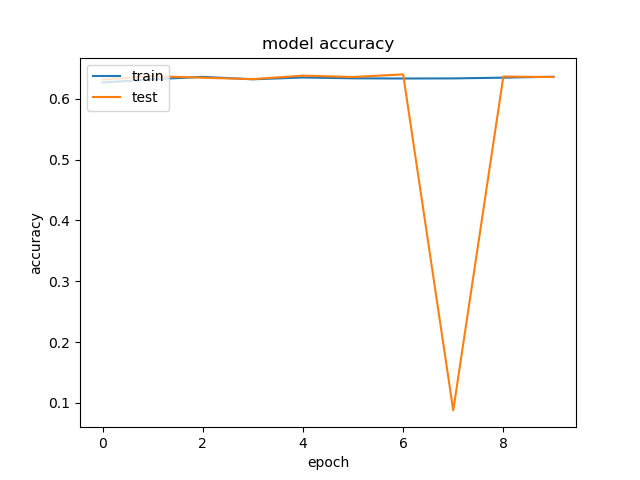
\includegraphics[width=1.2\linewidth]{img/pre-trained_models/Inception_v3_acc.png}
  \caption{Accuracy}
  \label{fig:sub1}
\end{subfigure}%
\begin{subfigure}{.5\textwidth}
  \centering
  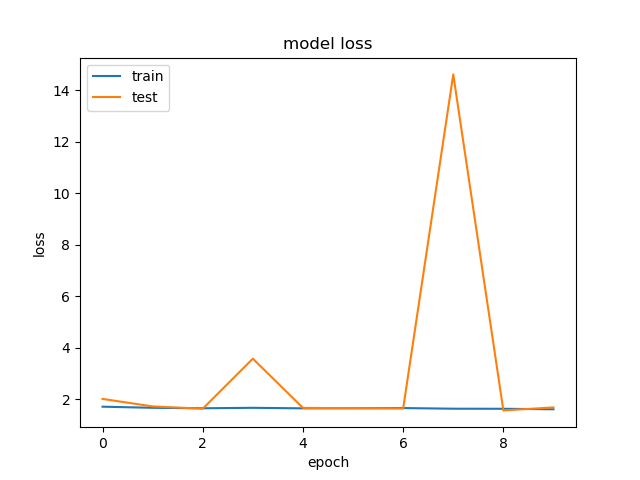
\includegraphics[width=1.2\linewidth]{img/pre-trained_models/Inception_v3_loss.png}
  \caption{Loss}
  \label{fig:sub2}
\end{subfigure}
\caption{Accuracy and loss after 10 epochs for the Inception V3 model with Imagenet initialization}
\label{fig:inception_v3_ten_epochs_imagenet}
\end{figure}


\begin{figure}[h!]
\centering
\begin{subfigure}{.5\textwidth}
  \centering
  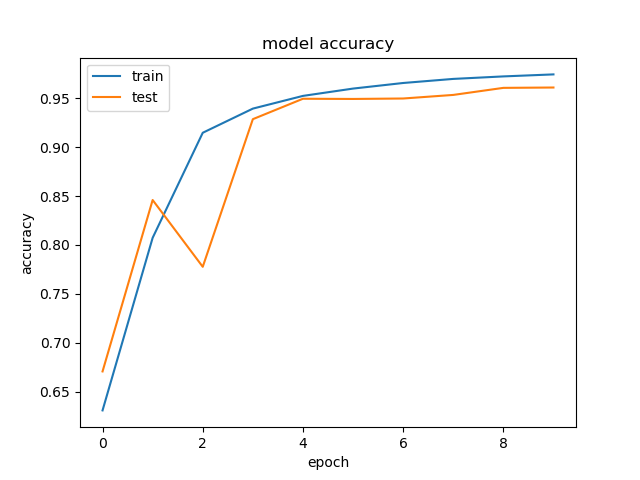
\includegraphics[width=1.2\linewidth]{img/pre-trained_models/vgg16_pretrained_acc.png}
  \caption{Accuracy}
  \label{fig:sub1}
\end{subfigure}%
\begin{subfigure}{.5\textwidth}
  \centering
  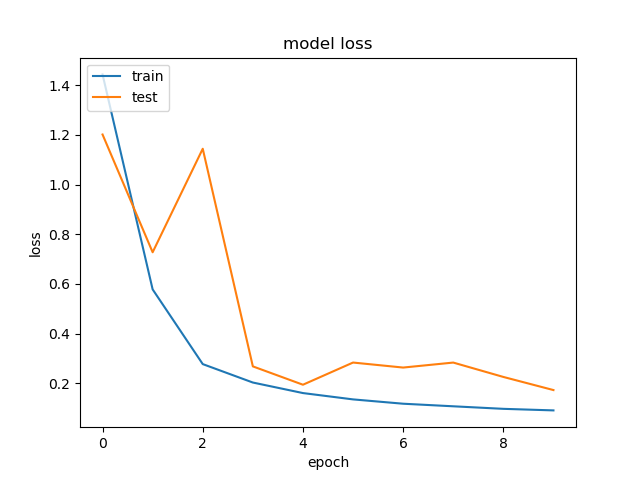
\includegraphics[width=1.2\linewidth]{img/pre-trained_models/vgg16_pretrained_loss.png}
  \caption{Loss}
  \label{fig:sub2}
\end{subfigure}
\caption{Accuracy and loss after 10 epochs for the VGG16 model with Imagenet initialization}
\label{fig:vgg16_ten_epochs_imagenet}
\end{figure}


\begin{figure}[h!]
\centering
\begin{subfigure}{.5\textwidth}
  \centering
  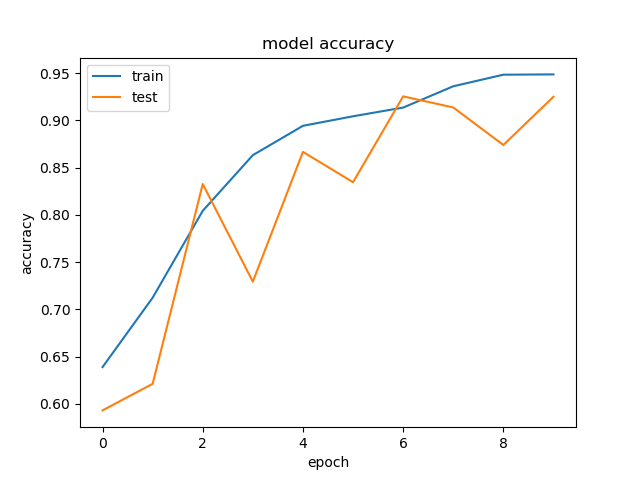
\includegraphics[width=1.2\linewidth]{img/pre-trained_models/ResNet50_pretrained_acc.png}
  \caption{Accuracy}
  \label{fig:sub1}
\end{subfigure}%
\begin{subfigure}{.5\textwidth}
  \centering
  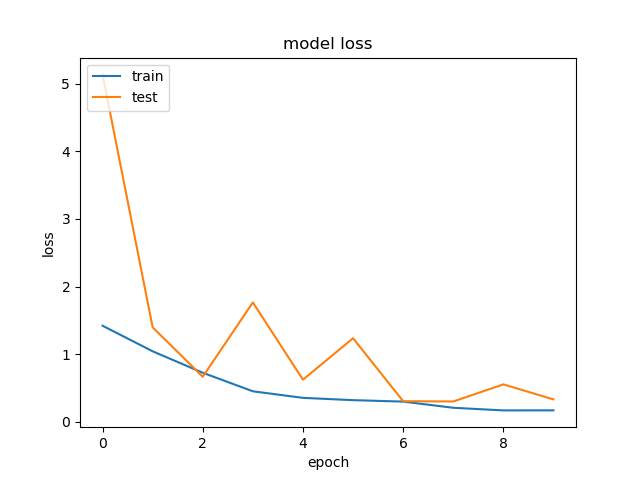
\includegraphics[width=1.2\linewidth]{img/pre-trained_models/ResNet50_pretrained_loss.png}
  \caption{Loss}
  \label{fig:sub2}
\end{subfigure}
\caption{Accuracy and loss after 10 epochs for the ResNet50 model with Imagenet initialization}
\label{fig:resnet50_ten_epochs_imagenet}
\end{figure}


The experiments show that there is no initial boost in training accuracy when the CNN models are initialized with pre-trained ImageNet weights. This fact is more obviously shown in table \ref{tab:one_epoch_xavier_vs_imagenet} with the initial accuracy values after one epoch for both initialization strategies.


\begin{table}[h!]
\center
\begin{tabular}{|l|l|l|l|l|l|}
\hline
\textbf{Model} & \textbf{Xavier init acc} & \textbf{ImageNet init acc}\\ \hline
 Inception V3	& 0.6539  & 0.6268\\ \hline
 VGG16  		& 0.6519  	 	 &  0.6307	  	\\ \hline     
 ResNet50  	& 0.6916  	  	 & 0.6389\\ \hline
\end{tabular}
\caption{Accuracy comparison after one epoch with Xavier and ImageNet initialization}
\label{tab:one_epoch_xavier_vs_imagenet}
\end{table}


The final accuracy values for both initialization strategies are shown in table \ref{tab:10_epochs_xavier_vs_imagenet}. Only VGG16 achieved a slightly higher accuracy value at the end while using the ImageNet initialization strategy while the other two models performed worse.

\begin{table}[h!]
\center
\begin{tabular}{|l|l|l|l|l|l|}
\hline
\textbf{Model} & \textbf{Xavier init acc} & \textbf{ImageNet init acc}\\ \hline
 Inception V3	& 0.9338  & 0.6334\\ \hline
 VGG16  		& 0.9723  	 	 &  0.9745	  	\\ \hline     
 ResNet50  	&  0.9548 	  	 & 0.9134 \\ \hline
\end{tabular}
\caption{Accuracy comparison after 10 epochs with Xavier and ImageNet initialization}
\label{tab:10_epochs_xavier_vs_imagenet}
\end{table}



\newpage




\section{Discussion} \label{discussion}





The training accuracy did not start higher as expected but lower when using pre-trained ImageNet weights as the initialization strategy. The final training accuracy only improved slightly for one model, namely VGG16 while the other two models performed worse.\\
The main problem here is probably the naive approach to make all layers of the CNN models trainable. By making all layers trainable the idea behind transfer learning is almost lost because the trained weights of the other domain are overwritten by the inputs of the new domain. The initialization of weights from another domain than the target domain therefore probably leads to a weight distribution which is not ideal as an initialization approach and shifts too far from the distribution which needs to be learned.
The fact that all layers of the pre-trained CNN models have been made trainable leads to a longer and more costly error-correction process inside the networks while trying to correct the already learned basic ImageNet features to fit the new domain of spectrograms. This is probably the reason why the ImageNet initialization strategy leads to lower starting accuracies. A better approach to test if pre-trained ImageNet weights are beneficial to the task of keyword spotting would probably be to recursively "freeze" the layers of the chosen model which makes them untrainble and check which is the optimal amount of frozen layers which leads to the highest accuracy. The main approach to transfer learning is to use a certain amount of frozen or fixed layers which learned the weight distribution of another domain and then stack another shallow model on top which uses the already learned features while fine-tuning this top model. The shallow model on top which is called "standard top layer configuration" in this project is explained in section \ref{cnn_models} but is probably superfluous in this setup because all layers of the tested models are trainable and are therefore able to learn the new target domain based on their complexity. Another explanation could be that the setup is right but the originally learned domain of ImageNet inputs differs too much from the target domain of keyword spotting using log spectrograms.\\
The different CNN topologies indicate that pre-trained ImageNet weights are not a suitable initialization strategy when it comes to the presented task of keyword spotting because they all experienced the same effect of lower starting accuracies but on the other hand all layers of all CNN models have been made trainable which might negates the statement that pre-trained ImageNet weights are not suitable for this case.\\
Batch Normalization normalizes input per mini-batch and helps speeding up the training process but also makes the initialization strategy less important \cite{ioffe2015batch} which is a crucial point which has not been considered carefully enough before setting up the experiment. During the experiment a certain progress in convergence rate towards the accuracy maximum has been shown by using batch normalization but it might have been a better option to drop the batch normalization layers in favor of having clearer results about the initialization strategies and only use dropout as a regularization technique.\\
Adam as an optimization strategy may not be the best fit based on its initialization bias correction terms \cite{kingma2014adam}. Stochastic gradient descent may be the better fit because it has also been used in previos works in similar domains \cite{gouda2018speech} while other optimization strategies might also be worth investigating as long as they do not correct the initialization bias.\\

RGB data vs grayscale problem??????



\section{Conclusion}

The experiments have shown that the usage of pre-trained ImageNet weights as an initialization strategy for CNNs in order to tackle the task of keyword spotting using spectrograms is not beneficial but rather harmful. Unfortunately, the hypothesis that pre-trained ImageNet weights as an initialization strategy for the task of speech recognition would be beneficial could not be proven.\\

On the other hand, there is still room for improvement in terms of setup variables to disprove this statement by adjusting the transfer learning strategy by freezing different amounts of layers, using a different optimization strategy or using another generalization technique than batch normalization which is not influencing the importance of the initialization strategy as discussed in section \ref{discussion}.


\section{Future Work} \label{future_work}

Future work could concentrate on the effect of batch normalization with regards to transfer learning and in how far it influences the importance of the right initialization strategy.\\ 
Another point which is worth investigating is the right amount of fixed or frozen layers while applying transfer learning between domains which do not directly relate to each other like speech recognition and image classification as presented in this project. The right amount of fixed layers and how far fine-tuning has to be applied in order to make use of already learned features from another domain seems to be of great importance. The idea of recursive feature elimination as used in text analysis to determine the most contributing features could also be applied to the right amount of fixed or frozen layers.\\
Additional preprocessing and feature engineering steps also seem interesting to investigate when transfer learning is applied, e.g., the correlation between accuracy and the dimensions of spectrograms while using already learned features from another domain. The detection of outliers and removing bad audio samples could also be beneficial in order to boost the overall accuracy.\\
Using spectrograms based on other features like mel frequency cepstral coefficients (MFCC) and see if transfer learning is beneficial could also be an interesting area to investigate in the future.






% You can choose a citation style, 'plain' is the default
% See:
% https://www.overleaf.com/learn/latex/Bibtex_bibliography_styles

\bibliographystyle{plain}
\bibliography{references.bib}

\end{document}

% Have fun!
% -fons

% http://www2.washjeff.edu/users/rhigginbottom/latex/resources/symbols.pdf